\hypertarget{pf__daemon_8h}{
\section{pf\_\-daemon.h File Reference}
\label{pf__daemon_8h}\index{pf\_\-daemon.h@{pf\_\-daemon.h}}
}


This graph shows which files directly or indirectly include this file:\nopagebreak
\begin{figure}[H]
\begin{center}
\leavevmode
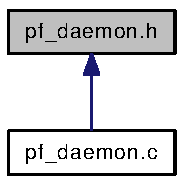
\includegraphics[width=62pt]{pf__daemon_8h__dep__incl}
\end{center}
\end{figure}
\subsection*{Defines}
\begin{CompactItemize}
\item 
\#define \hyperlink{pf__daemon_8h_551ae9e7796a78ff54bc98eef4e74498}{LOCKFILE}~\char`\"{}.lock\char`\"{}
\end{CompactItemize}
\subsection*{Functions}
\begin{CompactItemize}
\item 
void \hyperlink{pf__daemon_8h_0e2f72a981c64aefe314e745b28b6387}{start\_\-daemon} ()
\item 
void \hyperlink{pf__daemon_8h_725630dc6f9856b1349100761924050f}{stop\_\-daemon} ()
\item 
void \hyperlink{pf__daemon_8h_db0a9558ddd4dc0bbad7b5ddfc5231c6}{dbus\_\-listen} ()
\end{CompactItemize}


\subsection{Define Documentation}
\hypertarget{pf__daemon_8h_551ae9e7796a78ff54bc98eef4e74498}{
\index{pf\_\-daemon.h@{pf\_\-daemon.h}!LOCKFILE@{LOCKFILE}}
\index{LOCKFILE@{LOCKFILE}!pf_daemon.h@{pf\_\-daemon.h}}
\subsubsection{\setlength{\rightskip}{0pt plus 5cm}\#define LOCKFILE~\char`\"{}.lock\char`\"{}}}
\label{pf__daemon_8h_551ae9e7796a78ff54bc98eef4e74498}




Definition at line 1 of file pf\_\-daemon.h.

Referenced by start\_\-daemon(), and stop\_\-daemon().

\subsection{Function Documentation}
\hypertarget{pf__daemon_8h_db0a9558ddd4dc0bbad7b5ddfc5231c6}{
\index{pf\_\-daemon.h@{pf\_\-daemon.h}!dbus\_\-listen@{dbus\_\-listen}}
\index{dbus\_\-listen@{dbus\_\-listen}!pf_daemon.h@{pf\_\-daemon.h}}
\subsubsection{\setlength{\rightskip}{0pt plus 5cm}void dbus\_\-listen ()}}
\label{pf__daemon_8h_db0a9558ddd4dc0bbad7b5ddfc5231c6}


Function that provides method calls.

Bus name: to.networld.moksec.phonefirewall Object name: to.networld.moksec.phonefirewall.Object interface: to.networld.moksec.phonefirewall.Checking methods: checkblacklist(...) checkwhitelist(...) \hypertarget{pf__daemon_8h_0e2f72a981c64aefe314e745b28b6387}{
\index{pf\_\-daemon.h@{pf\_\-daemon.h}!start\_\-daemon@{start\_\-daemon}}
\index{start\_\-daemon@{start\_\-daemon}!pf_daemon.h@{pf\_\-daemon.h}}
\subsubsection{\setlength{\rightskip}{0pt plus 5cm}void start\_\-daemon ()}}
\label{pf__daemon_8h_0e2f72a981c64aefe314e745b28b6387}


Starts the program as a daemon and creates a lockfile (specified in the LOCKFILE constant). So it's impossible to start the daemon twice. \hypertarget{pf__daemon_8h_725630dc6f9856b1349100761924050f}{
\index{pf\_\-daemon.h@{pf\_\-daemon.h}!stop\_\-daemon@{stop\_\-daemon}}
\index{stop\_\-daemon@{stop\_\-daemon}!pf_daemon.h@{pf\_\-daemon.h}}
\subsubsection{\setlength{\rightskip}{0pt plus 5cm}void stop\_\-daemon ()}}
\label{pf__daemon_8h_725630dc6f9856b1349100761924050f}


Stops the daemon and deletes the lockfile, so a new instance can be started. 